\chapter{The Dynamics of Learning: Fitting vs. Compression}
\label{ch:learning_dynamics}

The training of deep neural networks is often viewed in practice as a monolithic optimization process: we define a loss function, initialize parameters, and descend the loss landscape until convergence. From this perspective, the goal is simply to minimize empirical error. However, when we analyze this process through the lens of information theory---specifically by tracking the information flowing through the hidden layers---a rich, multi-phase dynamic emerges. This chapter explores the phenomenon of learning dynamics by examining the trajectory of a neural network in the \textit{Information Plane}, revealing how the mutual information between the representations, the inputs, and the targets evolves over time.

% 1. Descriptive Opening
\section{The Two Phases of Stochastic Gradient Descent}

In traditional machine learning, empirical risk minimization (ERM) provides the fundamental framework for understanding learning. ERM guarantees that minimizing training loss with appropriate regularization will, under certain conditions, lead to generalization on unseen data. Yet, ERM says little about the structure of the internal representations learned by the network. Why do deep architectures generalize so well despite being heavily overparameterized? What happens to the features encoded in the hidden layers as training progresses?

In 2017, Shwartz-Ziv and Tishby proposed a radical reinterpretation of deep learning dynamics based on the Information Bottleneck (IB) principle (introduced in Chapter 8). By treating the sequential layers of a neural network as a Markov chain:
\begin{equation}
    Y \leftrightarrow X \rightarrow Z_1 \rightarrow Z_2 \rightarrow \dots \rightarrow Z_L \rightarrow \hat{Y}
\end{equation}
they tracked the optimization process by projecting each layer $Z_l$ onto a two-dimensional space called the Information Plane. The coordinates of this plane are defined by two key mutual information quantities:
\begin{enumerate}
    \item $I(X; Z_l)$: The information the layer retains about the input data. This represents the \textit{complexity}, or the memory capacity, of the representation. 
    \item $I(Z_l; Y)$: The information the layer contains about the target label. This represents the \textit{predictive power}, or the task-relevant accuracy, of the representation.
\end{enumerate}

Empirically observing the trajectories of neural networks trained with Stochastic Gradient Descent (SGD) on this plane, Tishby and colleagues identified that the optimization process naturally splits into two distinct and successive phases.

\textbf{Phase I: The Fitting Phase.} During the initial epochs of training, the network experiences large, coherent gradients. The parameters move rapidly down the steepest slopes of the loss landscape. In this phase, the network acts as an information sponge. It rapidly memorizes features from the input $X$ to correctly classify the training examples, driving the empirical loss down quickly. In the Information Plane, this corresponds to a sharp increase in $I(Z_l; Y)$ as predictive accuracy improves. Concurrently, $I(X; Z_l)$ also increases rapidly. The network builds a highly informative, albeit highly redundant and potentially overfitted, representation of the input. The signal (the true gradient of the loss) strongly dominates the noise (the stochasticity from mini-batch sampling).

\textbf{Phase II: The Compression Phase.} As the network approaches a local minimum of the empirical loss, the magnitude of the mean gradient diminishes significantly. The optimization dynamics shift. The coherent drift towards the minimum gives way to a stochastic random walk governed by the noise inherent in SGD's mini-batch sampling. Under the constraints of the data manifold, this diffusion causes the network weights to fluctuate. Crucially, these fluctuations act as an implicit regularization mechanism, causing the network to ``forget'' irrelevant, nuisance details of the input. In the Information Plane, this is observed as a slow, gradual decrease in $I(X; Z_l)$, while the predictive information $I(Z_l; Y)$ remains stable or slightly improves. The representation is effectively being compressed, discarding information that is not strictly necessary for the task.

This two-phase dynamic suggests a profound conclusion: SGD is not merely an optimization algorithm, but an implicit Information Bottleneck regularizer. The compression phase essentially performs the IB optimization---minimizing $I(X; Z_l)$ subject to maintaining $I(Z_l; Y)$---without any explicit regularization term in the loss function. The network discovers minimal sufficient statistics simply by wandering in the flat minima of the loss landscape. 

To understand the mechanics of this phenomenon, we must transition from a purely descriptive view to a rigorous mathematical formulation of SGD's stochastic dynamics.

% 2. Mathematical Core
\section{Mathematical Formalization of the Information Plane Dynamics}

We analyze a deep neural network parameterized by a vector $\theta \in \mathbb{R}^d$. Let the mapping from the input to the $l$-th hidden layer be given by a deterministic function $Z = f_\theta(X)$. 

\begin{figure}[htbp]
    \centering
    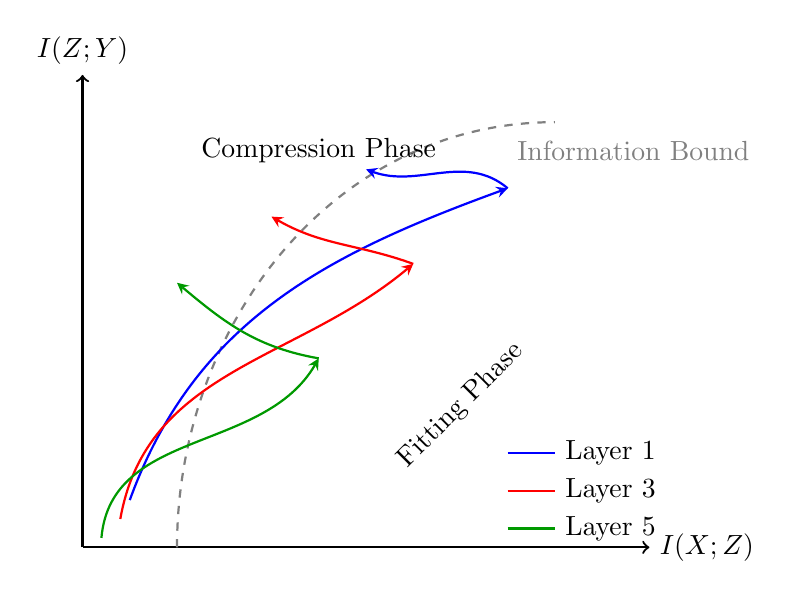
\begin{tikzpicture}[scale=1.2]
        % Axes
        \draw[->, thick] (0,0) -- (6,0) node[right] {$I(X; Z)$};
        \draw[->, thick] (0,0) -- (0,5) node[above] {$I(Z; Y)$};
        
        % Information bound curve
        \draw[thick, dashed, gray] (1,0) to[out=90, in=180] (5, 4.5);
        \node[gray, right] at (4.5, 4.2) {Information Bound};

        % Trajectories
        % Layer 1
        \draw[thick, blue, ->, >=stealth] (0.5, 0.5) to[out=70, in=200] (4.5, 3.8);
        \draw[thick, blue, ->, >=stealth] (4.5, 3.8) to[out=140, in=340] (3.0, 4.0);
        
        % Layer 3
        \draw[thick, red, ->, >=stealth] (0.4, 0.3) to[out=80, in=220] (3.5, 3.0);
        \draw[thick, red, ->, >=stealth] (3.5, 3.0) to[out=160, in=330] (2.0, 3.5);
        
        % Layer 5
        \draw[thick, green!60!black, ->, >=stealth] (0.2, 0.1) to[out=85, in=240] (2.5, 2.0);
        \draw[thick, green!60!black, ->, >=stealth] (2.5, 2.0) to[out=170, in=320] (1.0, 2.8);
        
        % Phase labels
        \node at (4.0, 1.5) [rotate=45] {Fitting Phase};
        \node at (2.5, 4.2) {Compression Phase};
        
        % Legend
        \draw[blue, thick] (4.5, 1.0) -- (5.0, 1.0) node[right, text=black] {Layer 1};
        \draw[red, thick] (4.5, 0.6) -- (5.0, 0.6) node[right, text=black] {Layer 3};
        \draw[green!60!black, thick] (4.5, 0.2) -- (5.0, 0.2) node[right, text=black] {Layer 5};
    \end{tikzpicture}
    \caption{Idealized trajectories of hidden layers in the Information Plane. Early in training, layers exhibit a fitting phase where they increase both $I(X;Z)$ and $I(Z;Y)$. As training progresses, they enter a compression phase, moving leftwards to decrease $I(X;Z)$ while maintaining $I(Z;Y)$.}
    \label{fig:info_plane}
\end{figure}

The update rule for SGD with learning rate $\eta$ and mini-batch size $B$ at iteration $t$ is defined as:
\begin{equation}
    \theta_{t+1} = \theta_t - \eta \nabla_\theta \hat{\mathcal{L}}_B(\theta_t)
\end{equation}
where $\hat{\mathcal{L}}_B(\theta) = \frac{1}{B} \sum_{i=1}^B \mathcal{L}(f_\theta(x_i), y_i)$ is the empirical loss computed over the current mini-batch drawn uniformly from the dataset $\mathcal{D}$. 

We can decompose the mini-batch gradient into the true full-batch gradient and an additive noise term:
\begin{equation}
    \nabla_\theta \hat{\mathcal{L}}_B(\theta_t) = \nabla_\theta \mathcal{L}(\theta_t) + \xi_t
\end{equation}
By the Central Limit Theorem, assuming $B$ is sufficiently large, the noise vector $\xi_t$ is approximately multivariate Gaussian with mean zero and a position-dependent covariance matrix $\Sigma(\theta_t) \approx \frac{1}{B} \text{Cov}_{x,y}[\nabla_\theta \mathcal{L}(f_\theta(x), y)]$.

This formulation allows us to model discrete SGD as a continuous-time Stochastic Differential Equation (SDE), specifically representing Langevin dynamics:
\begin{equation}
    d\theta_t = -\eta \nabla_\theta \mathcal{L}(\theta_t) dt + \sqrt{\eta \Sigma(\theta_t)} dW_t
\end{equation}
where $W_t$ represents a standard multi-dimensional Wiener process (Brownian motion). 

\subsection{The Drift-to-Diffusion Transition}

To mathematically define the boundary between the fitting and compression phases, we examine the Signal-to-Noise Ratio (SNR) of the gradients during training. The ``signal'' is the squared norm of the expected gradient drift, and the ``noise'' is given by the trace of the covariance matrix.

\begin{definition}[Signal-to-Noise Ratio of SGD]
    The gradient SNR at training time $t$ is defined as:
    \begin{equation}
        \text{SNR}(t) = \frac{\|\nabla_\theta \mathcal{L}(\theta_t)\|^2}{\frac{1}{d} \text{tr}(\Sigma(\theta_t))}
    \end{equation}
\end{definition}

\begin{figure}[htbp]
    \centering
    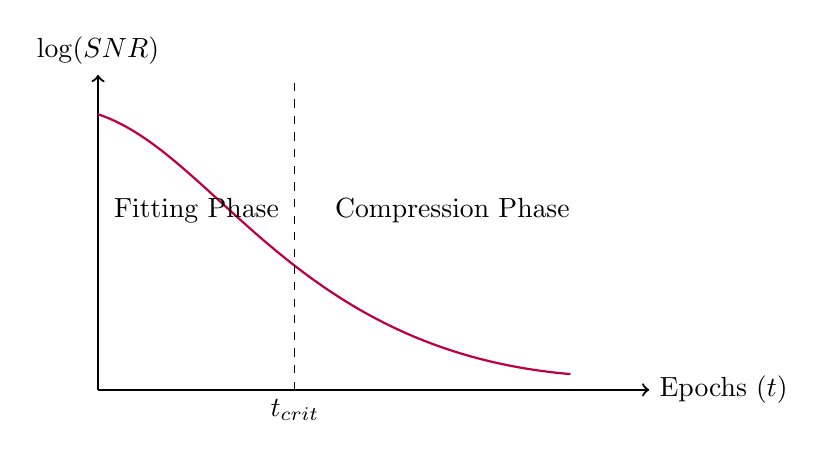
\begin{tikzpicture}[scale=1.0]
        \draw[->, thick] (0,0) -- (7,0) node[right] {Epochs ($t$)};
        \draw[->, thick] (0,0) -- (0,4) node[above] {$\log(\text{SNR})$};
        
        \draw[thick, purple] (0, 3.5) .. controls (1.5, 3.0) and (2.5, 0.5) .. (6, 0.2);
        
        \draw[dashed] (2.5, 0) -- (2.5, 4);
        \node[above] at (1.25, 2.0) {Fitting Phase};
        \node[above] at (4.5, 2.0) {Compression Phase};
        \node[below] at (2.5, 0) {$t_{\text{crit}}$};
    \end{tikzpicture}
    \caption{The transition from drift-dominated (fitting) to diffusion-dominated (compression) dynamics, marked by a critical, rapid drop in gradient SNR.}
    \label{fig:snr_drop}
\end{figure}

During the \textbf{Fitting Phase} ($t < t_{\text{crit}}$), the network parameters are far from any local minimum. The gradient magnitude is consequently large, yielding $\text{SNR} \gg 1$. The deterministic drift term $-\eta \nabla_\theta \mathcal{L}(\theta_t) dt$ dominates the SDE, rapidly driving the loss down and increasing $I(Z; Y)$.

During the \textbf{Compression Phase} ($t > t_{\text{crit}}$), the network enters a wide, flat region of the loss landscape (a ``flat minimum'') where $\nabla_\theta \mathcal{L}(\theta_t) \approx 0$. Consequently, the SNR drops exponentially. The stochastic diffusion term $\sqrt{\eta \Sigma(\theta_t)} dW_t$ now dominates the dynamics. The weights undergo a constrained random walk characterized by the noise covariance.

\subsection{Information Compression via Diffusion}

We now rigorously prove that this diffusion process inherently causes a decrease in the mutual information $I(X; Z)$. We restrict our analysis to a single hidden layer whose output is given by $Z = \phi(W X)$, where $\phi$ is a bounded, smooth activation function (such as $\tanh$ or the sigmoid function). For simplicity, we isolate the weight matrix $W$ of this specific layer, and assume the inputs $X$ are deterministic conditional on the sampled data.

\begin{theorem}[Information Compression via Weight Diffusion]
    Let $Z_t = \phi(W_t X)$ where $\phi : \mathbb{R} \to \mathbb{R}$ is a continuous, bounded activation function applied element-wise. Assume that in the compression phase, $W_t$ undergoes an isotropic diffusion process $dW_t = \sqrt{2D} d\tilde{W}_t$, where $D$ is the diffusion coefficient and $\tilde{W}_t$ is standard Brownian motion. If the marginal differential entropy $h(Z_t)$ is bounded from above, the mutual information $I(X; Z_t)$ monotonically decreases over time for sufficiently large $t$.
\end{theorem}

\begin{proof}
    By definition, the mutual information between the continuous input and the representation is:
    \begin{equation}
        I(X; Z_t) = h(Z_t) - h(Z_t | X)
    \end{equation}
    Because the activation function $\phi$ is bounded, the representation vector $Z_t$ is constrained to a compact hypercube (e.g., $[-1, 1]^k$). Therefore, by the principle of maximum entropy, the marginal differential entropy $h(Z_t)$ must be strictly bounded from above by some constant $h_{\text{max}}$.
    
    Now consider the conditional entropy $h(Z_t | X = x)$. For a fixed, constant input $x$, any randomness in $Z_t$ is induced entirely by the stochastic evolution of the weights $W_t$. 
    By applying Itô's Lemma, the diffusion of $W_t$ yields a corresponding diffusion process for the representation $Z_t$ conditional on $x$. Using a local linearization around the initial point of the diffusion $W_0$, we have:
    \begin{equation}
        Z_t \approx \phi(W_0 x) + J_x (W_t - W_0)
    \end{equation}
    where $J_x = \frac{\partial Z}{\partial W}\big|_{W=W_0}$ is the Jacobian matrix evaluated at $x$. Given that $W_t - W_0 \sim \mathcal{N}(0, 2DtI)$, the conditional distribution $P(Z_t | X=x)$ behaves asymptotically as a multivariate Gaussian with a covariance matrix $\Sigma_Z(t)$ that scales linearly with time:
    \begin{equation}
        \Sigma_Z(t) \approx 2 D t J_x J_x^T
    \end{equation}
    The differential entropy of a $k$-dimensional multivariate Gaussian is calculated as:
    \begin{equation}
        h(Z_t | X = x) = \frac{1}{2} \log \det (2 \pi e \Sigma_Z(t)) = \frac{k}{2} \log t + C(x)
    \end{equation}
    where $C(x)$ is a term dependent on the Jacobian $J_x$, the dimension $k$, and the diffusion constant $D$, but independent of time $t$.
    
    Taking the expectation over the data distribution $P(X)$ yields the overall conditional entropy:
    \begin{equation}
        h(Z_t | X) = \int P(x) h(Z_t | X=x) dx \approx \frac{k}{2} \log t + \mathbb{E}_X[C(X)]
    \end{equation}
    As $t \to \infty$ during the diffusion phase, the conditional entropy $h(Z_t | X)$ increases logarithmically without bound. 
    
    Since the marginal entropy $h(Z_t)$ remains bounded by $h_{\text{max}}$, it follows that the mutual information:
    \begin{equation}
        I(X; Z_t) = h(Z_t) - h(Z_t | X) \le h_{\text{max}} - \frac{k}{2} \log t - \mathbb{E}_X[C(X)]
    \end{equation}
    must necessarily decrease as time progresses. The persistent diffusion of the weights acts to ``blur'' the mapping from $X$ to $Z$, forcing the network to structurally forget high-resolution information about the input $X$.
\end{proof}

\subsection{Numerical Example}

To concretize this mechanism, consider a highly simplified setting: a scalar input $X \sim \mathcal{N}(0, 1)$ and a binary target $Y = \text{sgn}(X)$. We utilize a single-node hidden representation $Z = \tanh(w X)$ and a final output $\hat{Y} = \text{sgn}(v Z)$.

Suppose that at iteration $t_{100}$, marking the end of the fitting phase, the weight has reached $w = 5.0$. The mapping from $X$ to $Z$ is extremely sharp. 
\begin{align*}
    Z_{100} &= \tanh(5.0 X)
\end{align*}
Given $X=x$, $Z$ is nearly deterministic because the weights are temporarily stable. The variance of $Z|X$ is essentially zero, driving $h(Z_{100}|X) \to -\infty$ (for theoretical continuous weights) or reflecting extremely high precision. Evaluating this bounded mapping reveals that almost all information about $X$ is preserved up to the saturation regime, yielding $I(X; Z_{100}) \approx 0.95$ bits of the theoretical 1 bit maximum for this scale.

At iteration $t_{10000}$, deep in the compression phase, the weight $w$ has undergone extensive diffusion while remaining in the flat region solving the task. Its distribution might now be characterized by $w \sim \mathcal{N}(2.0, 1.5^2)$.
For a specific input, say $x=1.0$, the representation is $Z = \tanh(w)$ where $w$ is drawn from this Gaussian. The variance of $Z|X=1.0$ is now highly significant due to the variance in $w$. The conditional entropy $h(Z_{10000}|X)$ has therefore increased dramatically. A numerical integration of these distributions yields a substantially reduced mutual information $I(X; Z_{10000}) \approx 0.45$ bits. The representation has successfully compressed by shedding half a bit of information regarding the precise magnitude of $X$, while the decision boundary ($Z > 0 \implies \hat{Y} = 1$) remains perfectly intact, thus keeping $I(Z; Y)$ identical to its value in the fitting phase.

% 3. Horizon Box
\begin{horizon}
The universality and strict necessity of the compression phase remain topics of intense and active debate. While Shwartz-Ziv and Tishby observed compression robustly in networks equipped with saturating activation functions (such as $\tanh$ and sigmoid), subsequent seminal critiques (e.g., Saxe et al., 2018) fundamentally challenged the necessity of compression. They demonstrated that networks using ReLU activations often do not exhibit a distinct or visible compression phase in the Information Plane, yet these networks still generalize exceptionally well.

It is conjectured that for unbounded activation functions like ReLU, ``compression'' may not manifest as a reduction in differential entropy---which can scale arbitrarily through linear scaling of the weights---but rather through geometric clustering and a collapse in the intrinsic rank of the representations. Future work might show that the Information Plane, if augmented or normalized with invariant measures of intrinsic dimensionality, universally exhibits compression across all common architectures. A major open question is whether explicit informational compression (induced via noise) is causally responsible for robust generalization, or if it is merely a widespread epiphenomenon characteristic of stochastic optimization in high-dimensional spaces.
\end{horizon}

% 4. Summary and Exercises
\section{Summary}
\begin{itemize}
    \item The training dynamics of deep neural networks via SGD can be conceptually decomposed into a fast fitting phase and a slow compression phase when visualized on the Information Plane.
    \item This transition is characterized mathematically by a dramatic drop in the gradient Signal-to-Noise Ratio (SNR), marking a shift from drift-dominated optimization to diffusion-dominated random walks.
    \item In the compression phase, the stochastic noise inherent in SGD mini-batch sampling induces a random walk in parameter space. For bounded representations, this diffusion inherently increases the conditional entropy $h(Z|X)$ and drives a continuous decrease in the mutual information $I(X; Z)$, yielding compressed representations.
\end{itemize}

\section{Exercises}
\begin{enumerate}
    \item \textbf{Data Processing Inequality in the Plane:} Given the Markov chain sequence of layers $X \rightarrow Z_1 \rightarrow Z_2 \rightarrow Y$, formally prove that the trajectory of $Z_2$ in the Information Plane must always remain strictly below and to the left of the trajectory of $Z_1$.
    \item \textbf{Linear Networks and De Bruijn's Identity:} Consider a purely linear neural network layer defined by $Z_t = W_t X$. Show mathematically that if $W_t$ undergoes isotropic Gaussian diffusion, the conditional entropy $h(Z_t | X)$ increases, but the marginal entropy $h(Z_t)$ also increases indefinitely. Based on this result, conclude why saturating nonlinearities (or regularization) are necessary to observe true informational compression in this continuous SDE formulation.
    \item \textbf{Empirical Simulation:} Write a short Python script utilizing the \texttt{numpy} library to simulate the trajectory of a scalar weight $w_t$ undergoing SGD on the loss function $\mathcal{L}(w) = \frac{1}{4}(w^2 - 1)^2$. Inject artificial Gaussian noise to the gradient at each step. Plot the variance of $w_t$ over time after the weight reaches the local minimum at $w=1$, and observe the onset of the diffusion phase.
\end{enumerate}

% TODO-CITE: Ensure all named results are cited.
